\documentclass{ximera}

\graphicspath{{./graphics/}{./content/03_06_tangent_plane/graphics/}}

\title{Geometry of Differentiability}
\begin{document}
\begin{abstract}
\end{abstract}
\maketitle

In single variable calculus, derivatives were closely related to the slope of the tangent line to a graph at a point. We used this idea of the slope of the tangent line to define derivatives as a limit of slopes of secant lines,
\[
f'(a) = \lim_{h\rightarrow 0}\frac{f(a+h)-f(a)}{h}.
\]

\youtube{1FATfS-nTl8}

In the other direction, we were able to use differentiation rules to more easily find the equation for the tangent line to a graph at a point.

\begin{example}
We'll find the equation for the tangent line to the graph of $f(x)=x^3+2x+1$ at $x=2$.

We can find the slope of the tangent line by computing $f'(2)$. Using differentiation rules, we have
\[
f'(x) = \answer{3x^2+2}.
\]
Plugging in $x=2$, we have $f'(2) = \answer{14}$.

Since the tangent line will have to pass through the point $(2,f(2))$, we compute
\[
f(2) = \answer{13}.
\]

So, the tangent line will pass through the point $(2,13)$, and will have slope $14$. Writing the equation of the line in point-slope form, we have
\[
y-13 = \answer{14(x-2)}.
\]
\end{example}

When a single variable function is differentiable, we can use the above method to find an equation for the tangent line. In addition, the tangent line provides us with a good linear approximation for the function.

We would like to do something analogous for multivariable functions, but this raises a few questions. What would be the equivalent of the tangent line? What does it mean for a function to be differentiable?

As we begin to explore these questions, we'll focus on functions $\mathbb{R}^2\rightarrow\mathbb{R}$, so that we can visualize their graphs.

\section*{Geometric Interpretation of Differentiability}

In single variable calculus, we could get a good sense of whether a function was differentiable by looking at its graph.

\begin{problem}
For each of the graphs, determine whether the given function is differentiable at $x=a$.

\begin{image}
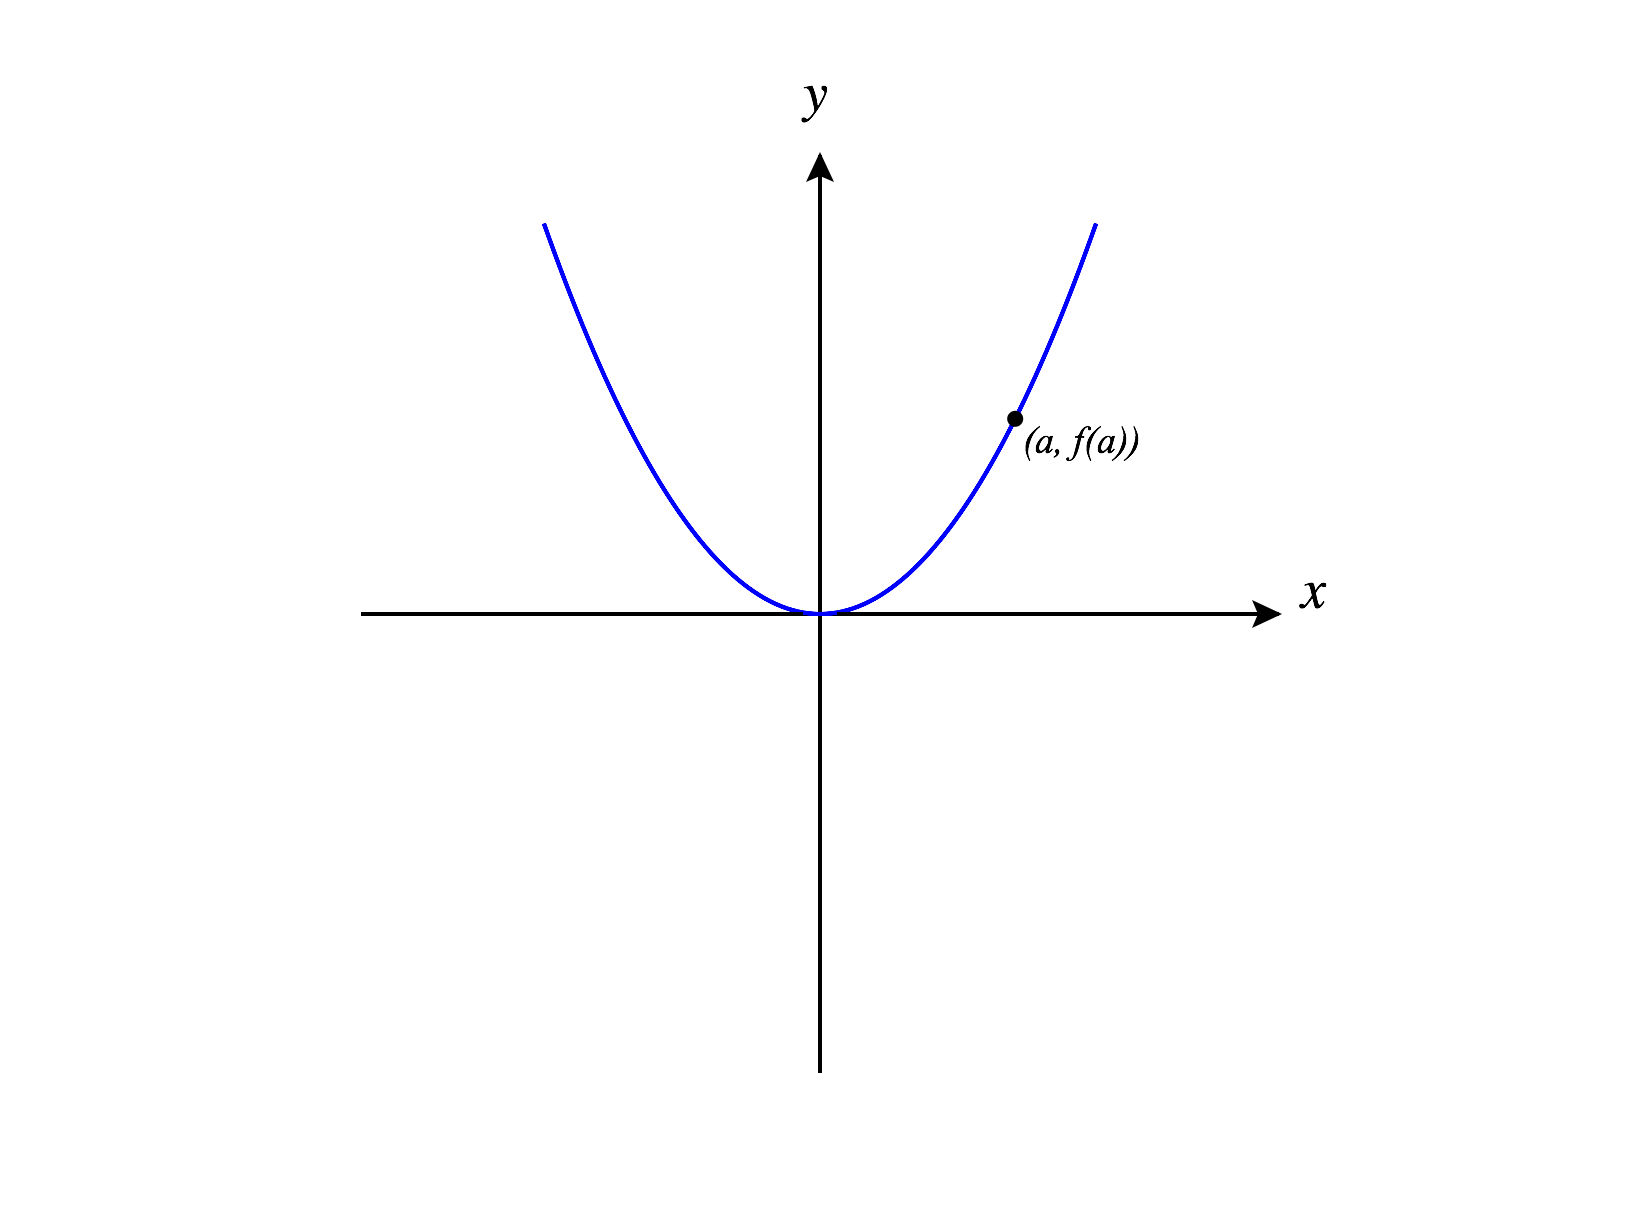
\includegraphics[width = \textwidth]{CalcPlot3D-sv_parabola}
\end{image}

\begin{multipleChoice}
\choice[correct]{differentiable}
\choice{not differentiable}
\end{multipleChoice}

\begin{image}
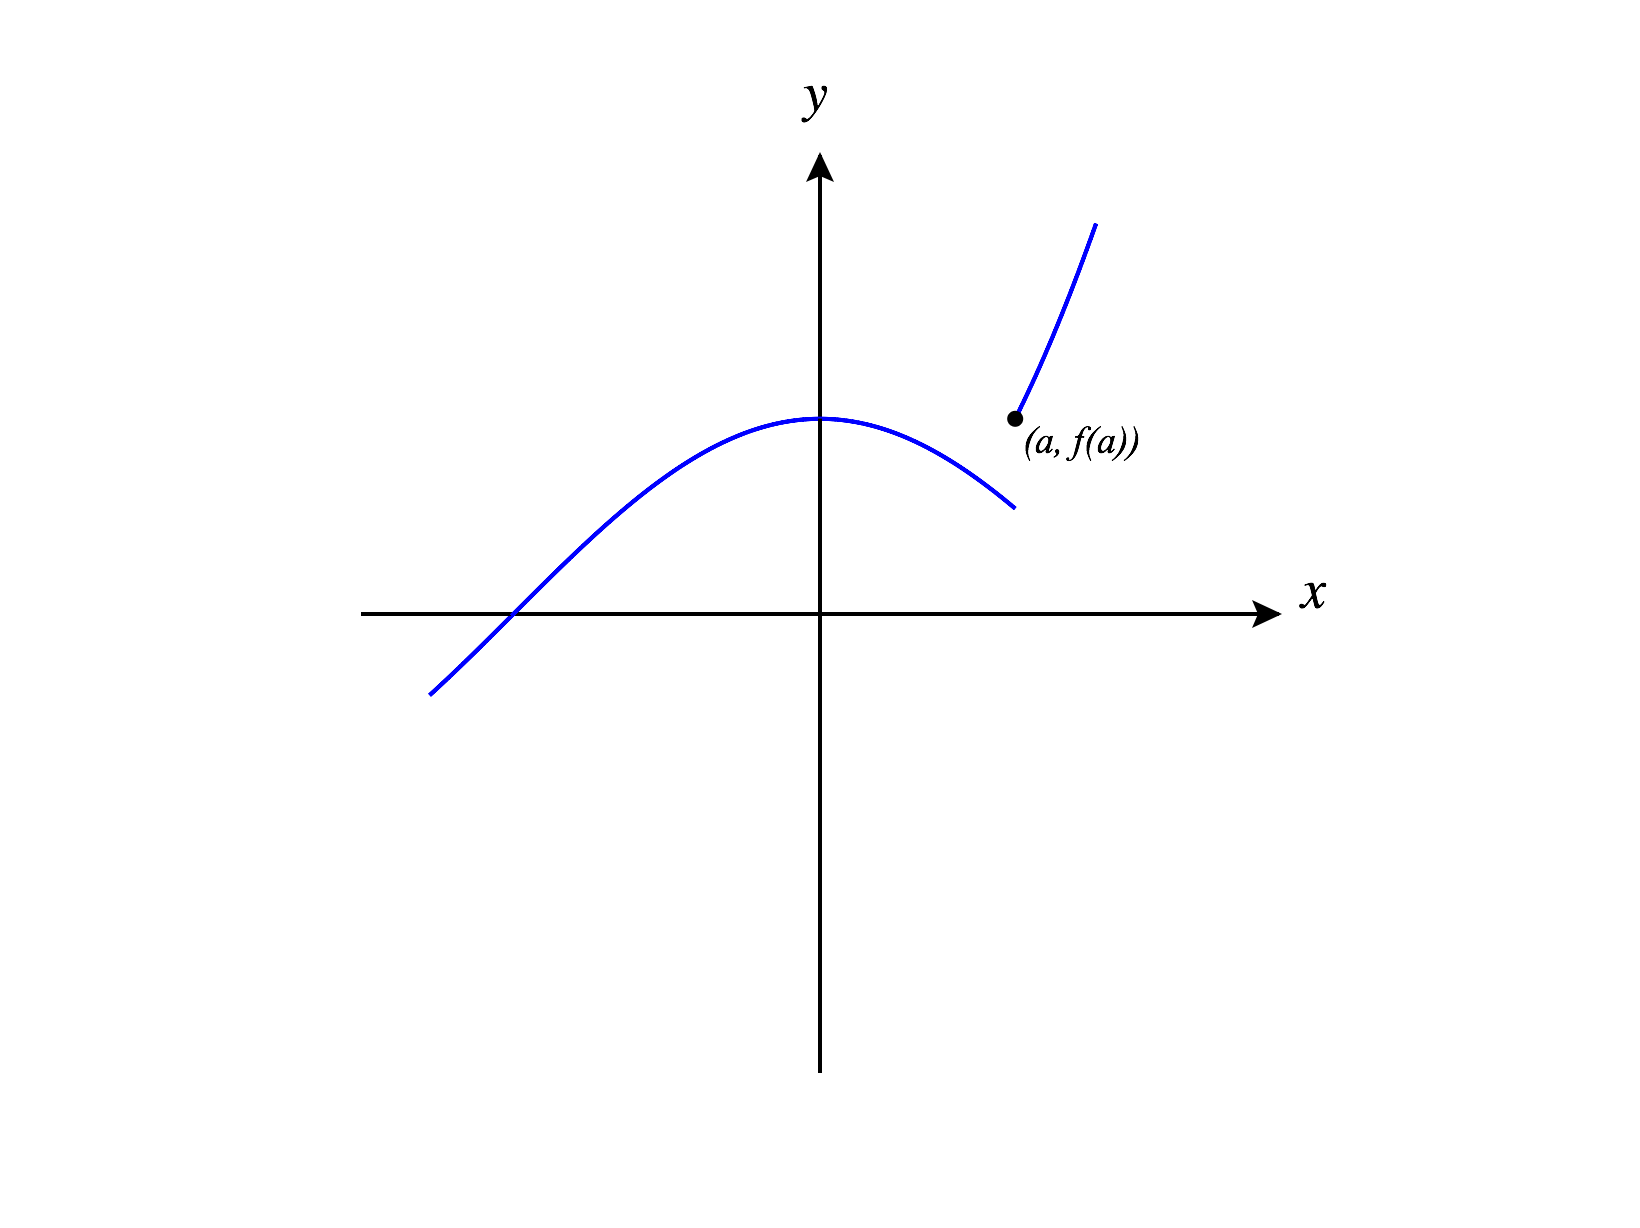
\includegraphics[width = \textwidth]{CalcPlot3D-sv_jump}
\end{image}

\begin{multipleChoice}
\choice{differentiable}
\choice[correct]{not differentiable}
\end{multipleChoice}

\begin{image}
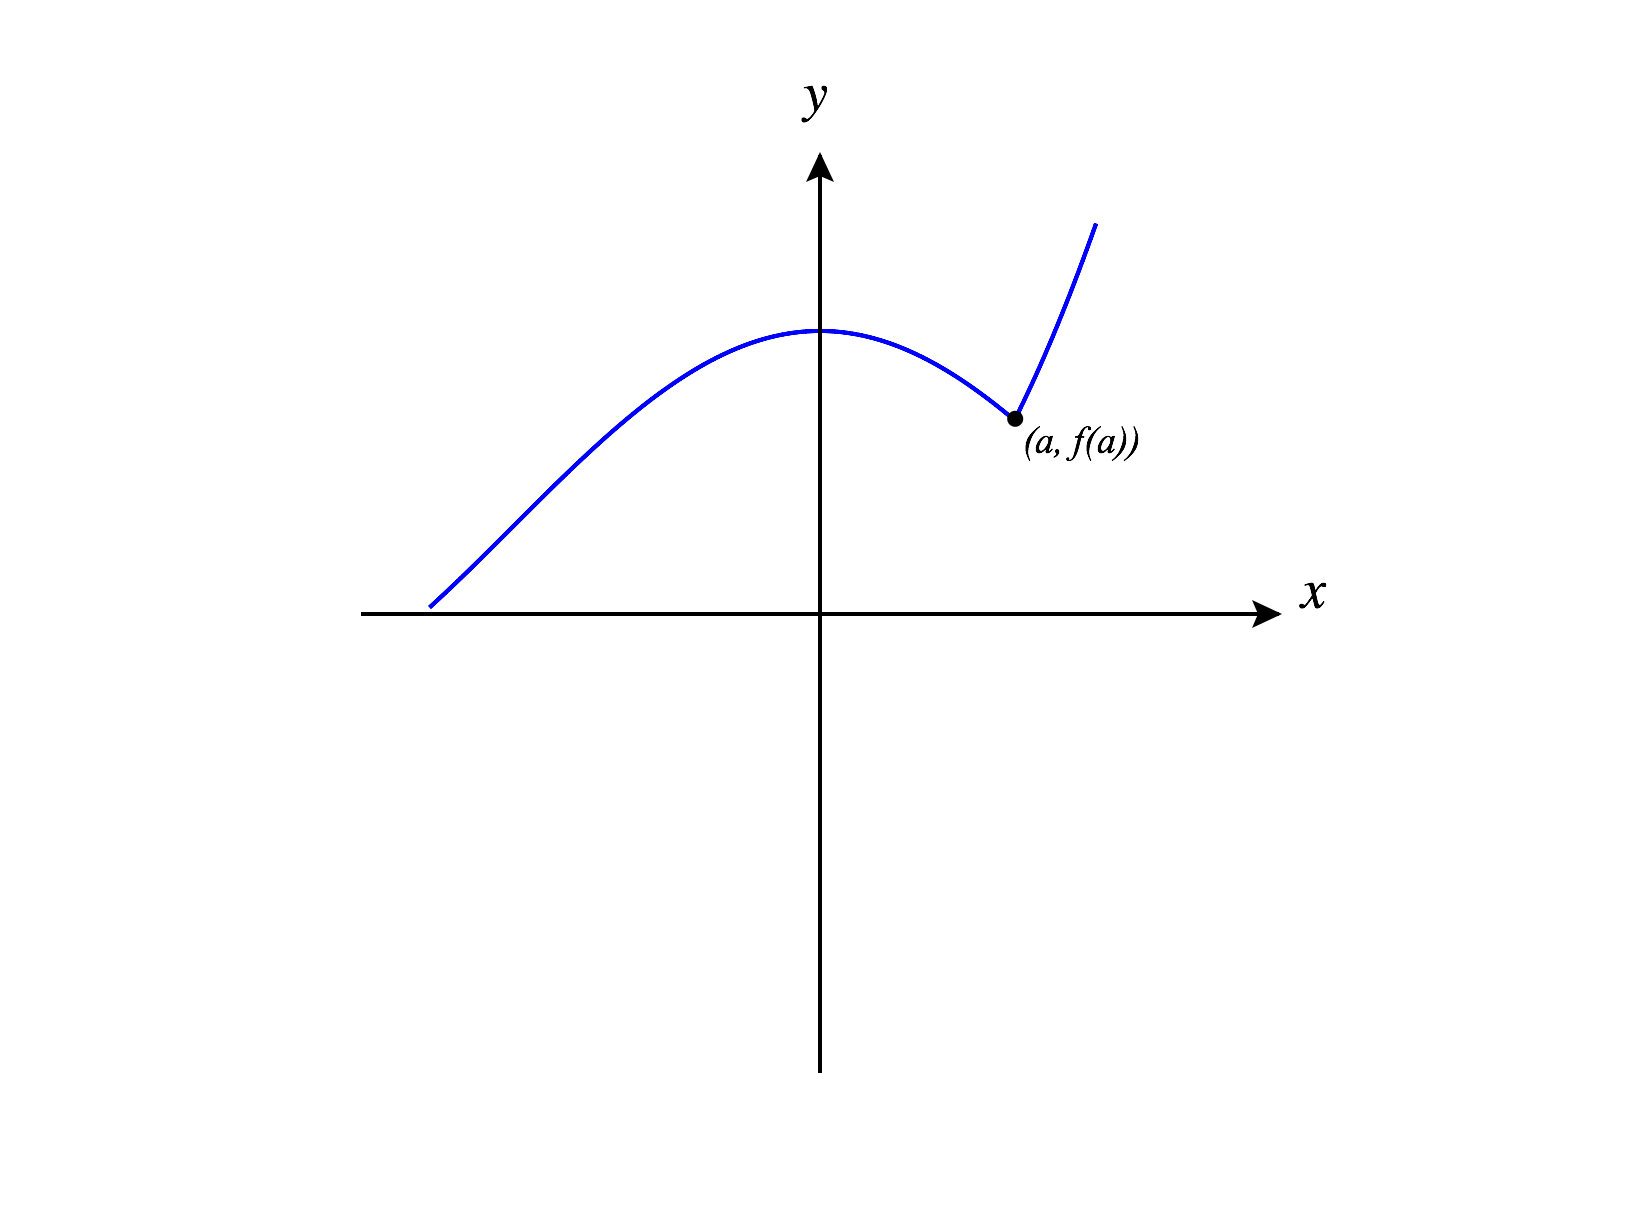
\includegraphics[width = \textwidth]{CalcPlot3D-sv_cusp}
\end{image}

\begin{multipleChoice}
\choice{differentiable}
\choice[correct]{not differentiable}
\end{multipleChoice}

\end{problem}

If there is a discontinuity or some sort of corner or cusp in the graph at a point, then the function will not be differentiable at that point. Roughly speaking, if we ``zoom in'' on the graph of a function near a point, and the graph looks very close to a line, then the function will be differentiable at that point.

\youtube{U_t2RFukDlA}

We'll extend this idea to make our first, informal definition of differentiability for a function from $\mathbb{R}^2$ to $\mathbb{R}$.

\begin{definition}
(Informal Definition) Consider a function $f:\mathbb{R}^2\rightarrow \mathbb{R}$. Suppose for some point $(a,b)$ in $\mathbb{R}^2$, if we zoom in on the graph of $f$ near the point $(a,b)$, the graph of $f$ looks like a plane. Then $f$ is differentiable at $(a,b)$.
\end{definition}

Although this definition provides us with nice geometric intuition for determining if a function is differentiable, it's not at all precise or rigorous. Eventually, we'll need a more formal definition of differentiability, so we'll return to this concept later.

For now, let's use this informal definition to investigate differentiability for a couple of functions.

\begin{example}
Consider the function $f(x,y) = xy+2x+y$, graphed below.

\youtube{AuaD1C1jLsA}

Is $f$ differentiable at $(0,0)$?
\begin{multipleChoice}
\choice[correct]{Yes.}
\choice{No.}
\end{multipleChoice}

\end{example}

\begin{example}
Consider the function 
\[
f(x,y) = \begin{cases} 
      1-|y| & \text{if }|y|\leq |x| \\
      1-|x| & \text{if }|y| > |x|
   \end{cases},
\] graphed below.

\youtube{u5CZGY65wtc}

Is f differentiable at $(0,0)$?
\begin{multipleChoice}
\choice{Yes.}
\choice[correct]{No.}
\end{multipleChoice}

\end{example}

\section*{The tangent plane}

If a function $f:\mathbb{R}^2\rightarrow\mathbb{R}$ is differentiable, when we zoom in, the graph will look like a plane. Because of this, there will be a plane that's a good linear approximation for the function near that point. We can use the partial derivatives with respect to $x$ and $y$ to find an equation for this plane, which we call the tangent plane.

\begin{definition}
If $f:\mathbb{R}^2\rightarrow\mathbb{R}$ is differentiable at $(a,b)$, then the \emph{tangent plane} to the graph of $f$ at $(a,b)$ is defined by the equation
\[
z=f(a,b)+f_x(a,b)(x-a)+f_y(a,b)(y-b).
\]
\end{definition}

Let's revisit our previous examples, and see what happens with the tangent plane.

\begin{example}
Consider the function $f(x,y) = xy+2x+y$, which we found is differentiable at the point $(0,0)$. Let's find an equation for the tangent plane to the graph of $f$ at $(0,0)$.

We begin by finding the partial derivatives with respect to $x$ and $y$.
\begin{align*}
f_x(x,y) &= \answer{y+2}\\
f_y(x,y) &= \answer{x+1}
\end{align*} 
At $(0,0)$, we have
\begin{align*}
f_x(0,0) &= \answer{2},\\
f_y(0,0) &= \answer{1}.
\end{align*} 
Finding the value of $f$ at $(0,0)$, we have
\[
f(0,0) = \answer{0}.
\]
Putting all of this together, we obtain an equation for the tangent plane to the graph of $f$ at $(0,0)$.
\begin{align*}
z &=f(a,b)+f_x(a,b)(x-a)+f_y(a,b)(y-b)\\
&= \answer{2x+y}
\end{align*}

\end{example}

\begin{example}
Consider the function 
\[
f(x,y) = \begin{cases} 
      1-|y| & \text{if }|y|\leq |x| \\
      1-|x| & \text{if }|y| > |x|
   \end{cases},
\] which we found is not differentiable $(0,0)$. Even though this function is not differentiable, let's see what happens when we try to find an equation for the tangent plane.

To compute the partial derivatives with respect to $x$ and $y$, we'll need to use the limit definition.

\begin{align*}
f_x(0,0) &= \lim_{h\rightarrow 0}\frac{f(0+h,0)-f(0,0)}{h}\\
&= \lim_{h\rightarrow 0}\frac{(1-|0|)-(1-|0|)}{h}\\
&= \lim_{h\rightarrow 0}\frac{0}{h}\\
&= 0\\
f_y(0,0) &= \lim_{h\rightarrow 0}\frac{f(0,0+h)-f(0,0)}{h}\\
&= \lim_{h\rightarrow 0}\frac{(1-|0|)-(1-|0|)}{h}\\
&= \lim_{h\rightarrow 0}\frac{0}{h}\\
&= 0
\end{align*}

We can also find $f(0,0)$,
\[
f(0,0)= 1.
\]

So, we have all of the necessary pieces to find an equation for the (nonexistent) ``tangent plane'':
\begin{align*}
z &=f(a,b)+f_x(a,b)(x-a)+f_y(a,b)(y-b)\\
&= 1.
\end{align*}

However, we decided that the function wasn't differentiable at $(0,0)$, so the graph does not have a tangent plane at the point.

\end{example}

This example brings up a couple of important points.
\begin{itemize}
\item It's possible for the partial derivatives of a function to all exist, and yet the function is not differentiable.
\item It's possible that we can find the equation $z =f(a,b)+f_x(a,b)(x-a)+f_y(a,b)(y-b)$, and yet $f$ has no tangent plane at the point $(a,b)$.
\end{itemize}

For these reasons, differentiability is a much more subtle concept in multivariable calculus than it was in single variable calculus, and our next task will be to find a formal definition for differentiability.



\end{document}